\section{Architecture}
\label{sec:arch}

\begin{figure}[!tb]
    \centering
    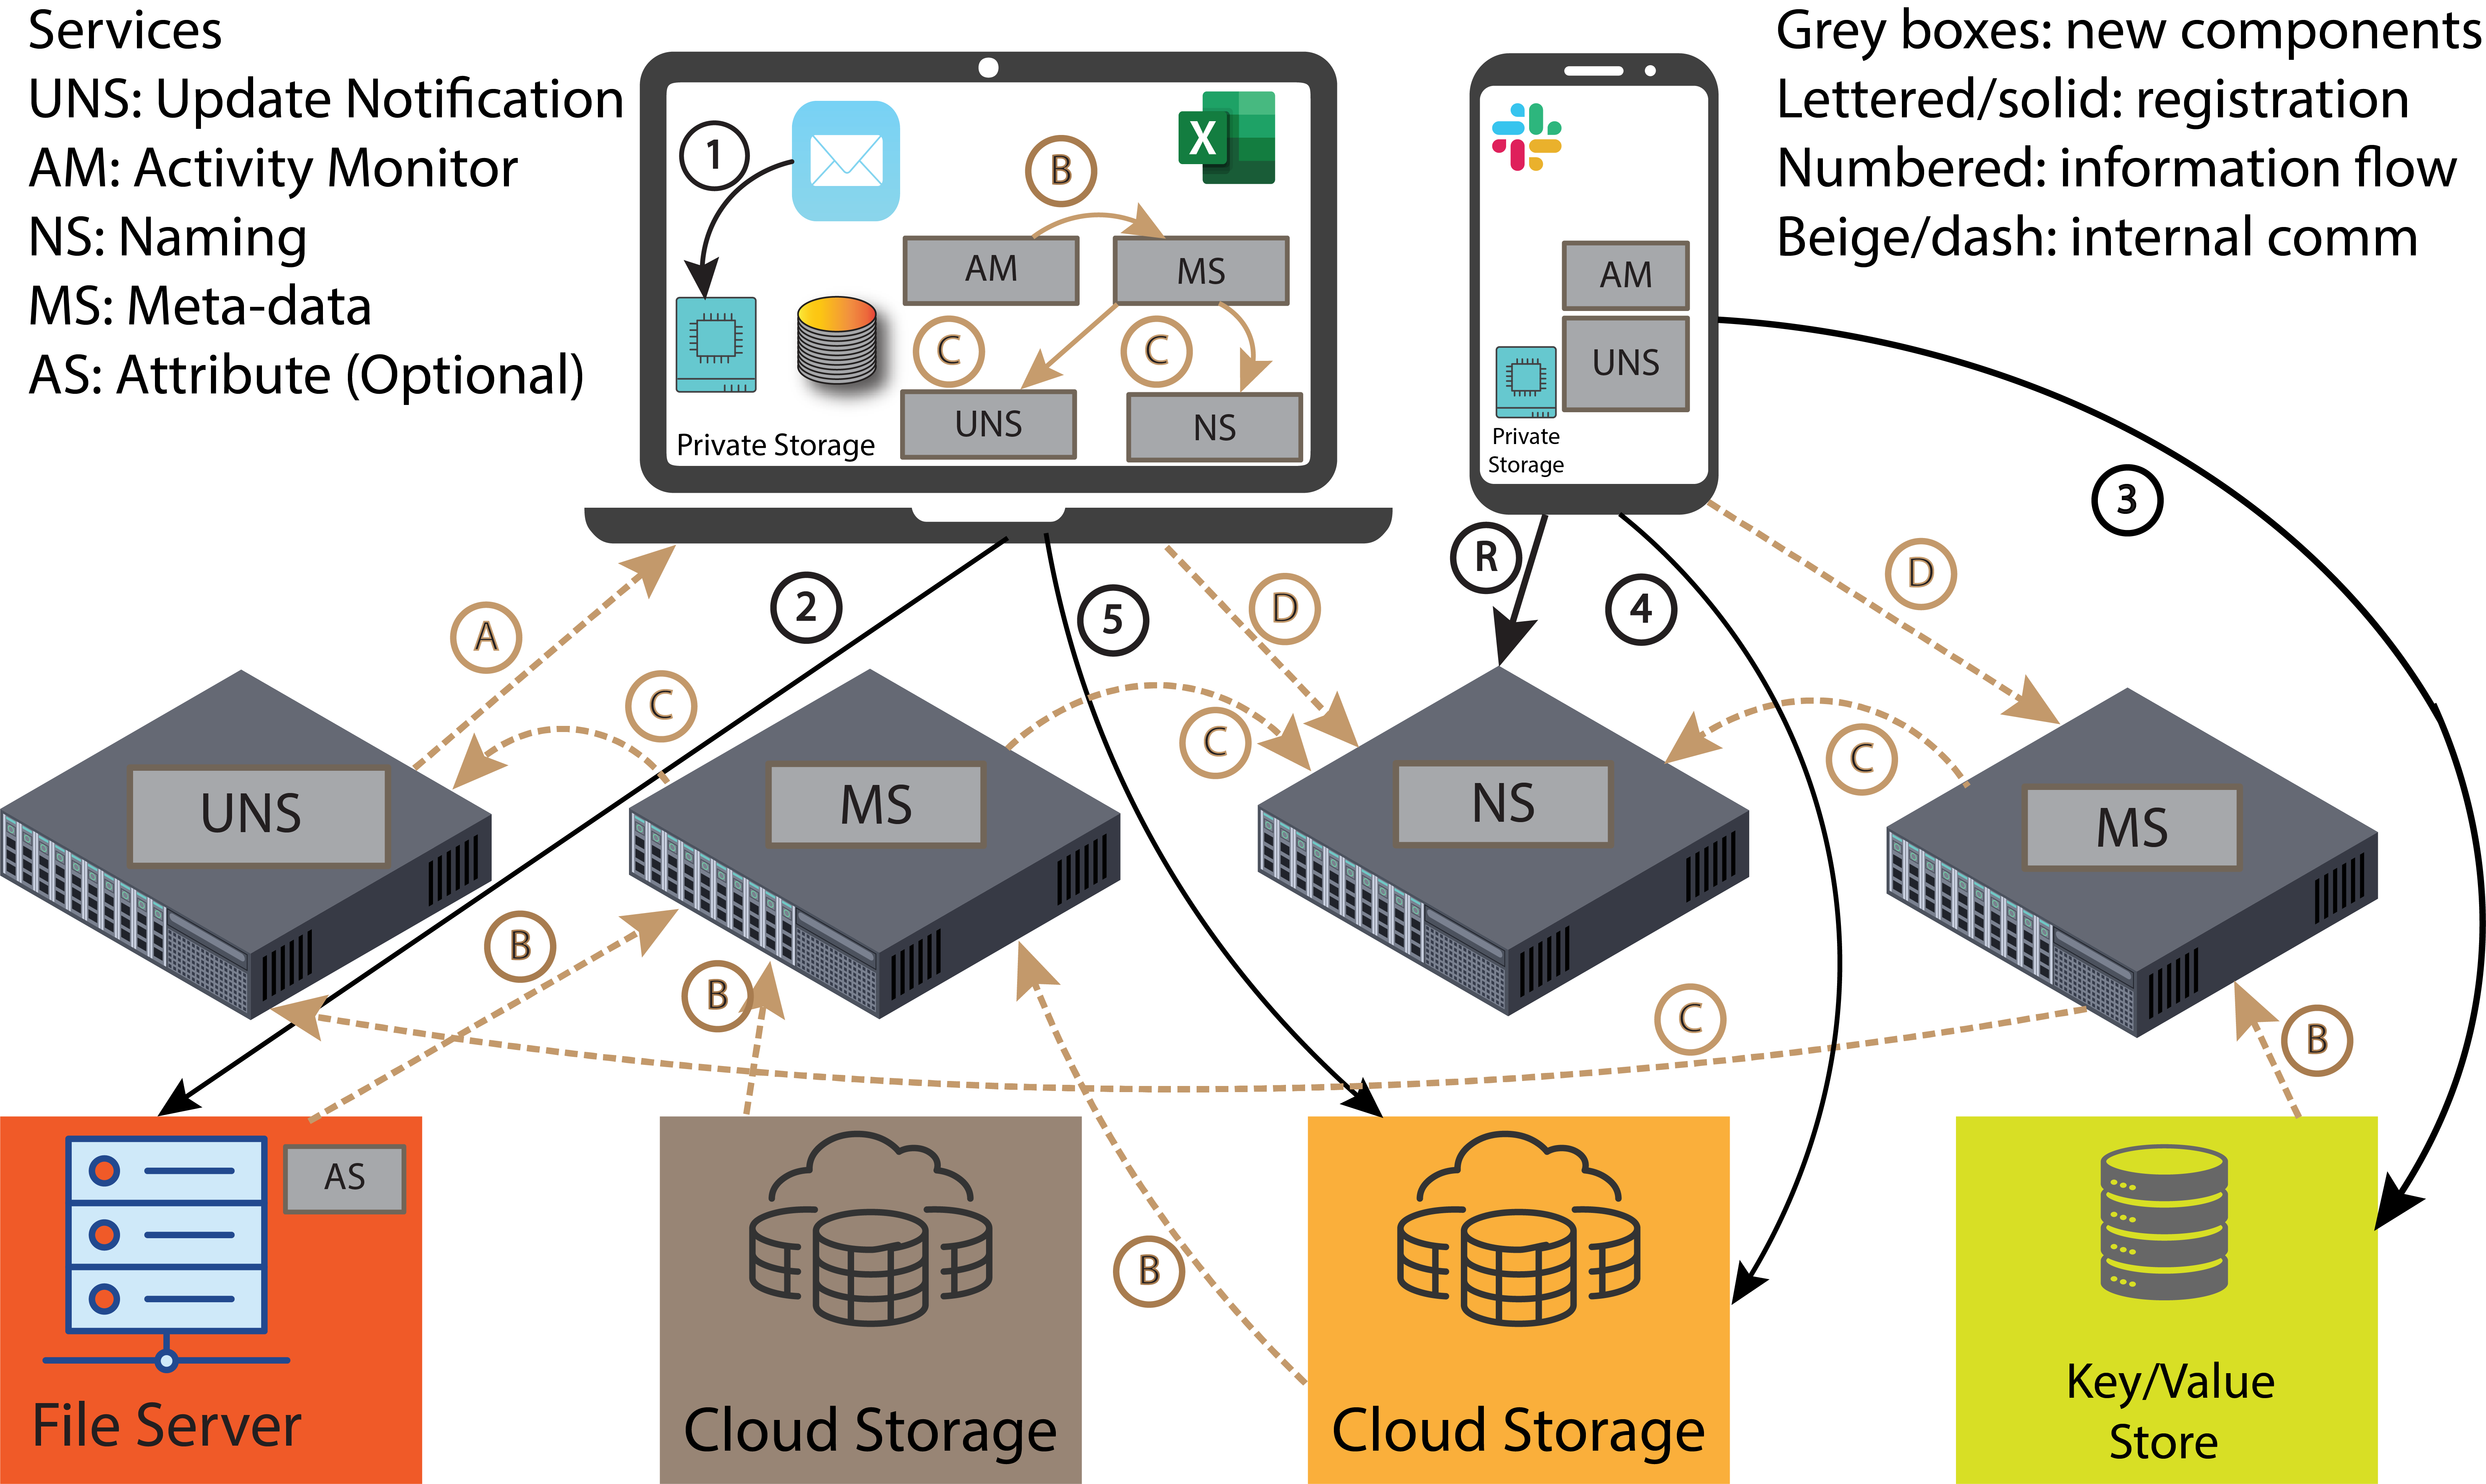
\includegraphics[width=0.45\textwidth]{figures/Naming5-legend.png}
    \caption{\system Architecture (\S \ref{sec:arch}).
    %Grey boxes indicate new components. AM=``Activity Monitor'', MS=``Meta-data Server'', UNS=``Update Notification Server'', NS=``Namespace Server''.
    }
    \label{fig:arch}
\end{figure}

%\reto{Using meta-data service that must inter-operate (federated meta data) and relationships are not first-class citizen, cannot glue the meta-data service together with naming services to enable the things we want to do. }
%\reto{the storage location is independent on the notion of related files: meta-data service treats relationships as first-class citizens. }
%\reto{get the attributes out of the silos --> currently: this is done manually}

\system is a family of services that enable sophisticated search and naming capabilities.
The key features that differentiate \system from prior work are: 
\textit{1)} incorporating object relationships as first class meta-data,
\textit{2)} federating meta-data services,
\textit{3)} recording activity context,
\textit{4)} integrating storage from multiple silos, and
\textit{5)} enabling customizable naming services.
Data continues to reside in existing and to-be-developed storage silos.
\system interacts with these silos, collects and captures metadata, and 
provides a federated network of metadata and naming services to
meet the needs of the use cases in \S \ref{sec:use-cases}.


\subsection{\system Services}

Figure \ref{fig:arch} illustrates the \system architecture. \system allows for different deployment scenarios. The five services can be run independently, they can be co-located and bundled together to run on a local device, integrated into an OS, or available as web-based services.
In the discussion below, parenthesized numbers and letters refer to the arrows in Figure \ref{fig:arch}.
There are five main components:

\noindent\textbf{1) Metadata servers (MS)}
are responsible for storing attributes and provide a superset of capabilities found in existing metadata services~\cite{federatedMetaData,smartstore}. Users can register an MS with activity monitors or attribute services, which allows the MS to receive updated attributes from storage objects and activities (B). Thus, there can be multiple sources of attributes including the user itself. Metadata servers may retain the full or partial history of attribute updates or maintain only the most recent value. 

\noindent\textbf{2) Namespace servers (NS)}
connect to one or more MS and use the metadata to provide users with a personalized namespace that allows both manual organization (i.e., a hierarchical namespace) and rich search capabilities. 
Users can register with an NS (R) that uses one or more MS to obtain relevant attributes from them (C). Additionally, users can be part of a corporate NS that allows sharing of their select metadata with other users via standard enterprise public-key cryptography.

\noindent\textbf{3) Activity monitors (AM)}
run on the user's devices. Their main function is to observe temporal relations, activity context, and relationships between objects on a user's device and transmit them to an MS (D).

\noindent\textbf{4) Attribute services (AS)}
extract attributes from storage objects and transmit them to an MS (B). An AS might be invoked on updates, run once or periodically. For example, a file system AS would update the object's metadata with basic attributes such as size or modification time. There can be many AS that extract more ``interesting'' attributes, e.g., image recognition, similarity, or other classifiers. 

\noindent\textbf{5) Update notification server (UNS)}
provides notification mechanisms. Users can register interest in changes of attributes or underlying storage and will receive a message on change events (A) to which they have access.

\subsection{\system working example}

To make the \system architecture concrete, we revisit our use-cases from \S\ref{sec:use-cases} and walk through parts of it to illustrate how \system supports the various actions and events. 

\noindent\textbf{Storing the e-mail attachment.}
\persa's act of saving the CSV file that \persc sent in email corresponds to the creation of a new object on the file server silo, i.e., the file system (4). The file server is \system-aware, so the AS co-located with it extracts attributes from the document and forwards them to the MS (B).

The AM on \persa's laptop detects that the CSV file came via company email from \persc. It then captures the activity context identifying the relationship between the e-mail and the CSV file and transmits it as additional metadata about the CSV file to the MS (that already contains metadata extracted by the AS). Moreover, because there is a company-wide namespace service, \system establishes that the e-mail attachment, the CSV in the file server, and the one on \persc's laptop (from which the file was sent) are exact copies of each other. 

Many applications already record some form of activity context, e.g., chat history, browsing history. Such histories provide a rich source of additional metadata. Other activity context, specifically the relationship between objects, such as the fact that a particular file was saved to a local storage device from an email message, requires more pervasive monitoring as found in, e.g., whole provenance capture systems~\cite{camflow}. \system is agnostic about the precise data that comprises activity context, but allows for storing and accessing activity context as metadata. 

\noindent\textbf{Creating the Excel file.}
Next, \persa opens the CSV file using Excel and stores it as a spread sheet. This creates a new object. The AM detects that the newly created spreadsheet is a conversion from the CSV file, either via a notification from \system-aware Excel or by monitoring the system calls executed on the local system. \persa proceeds to modify the data by filtering it in Excel and saving the changes. The AM records this event and updates the meta-data of the spreadsheet to record the derivation-relationship. Ideally a \system-aware version of Excel specifies to the AM the exact type of the relationship (in this case a derivation); otherwise the AM informs the MS about an unspecified data relationship by observing the opening of a CSV file and a subsequent creation of the Excel file. 

% \persa proceeds to upload the new Excel file on Slack, which triggers the creation of a new storage object as Slack creates a local copy, the addition of new metadata to MS via AS, and the addition of a \emph{copy} data relationship between the original Excel file and the Slack’s copy. The AM notices (by monitoring Slack chat) that the file was shared with user \persc and promptly notifies the MS, which adds this detail to its metadata. 

% Once \persa is done, its local MS has been updated with three new objects: the CSV file, the corresponding Excel file, and Slack’s copy of the Excel file. There is a data relationship linking all three, and the metadata informing us that the original CSV came from \persc and that the final Excel file was also shared with that same person. If \persa wanted to remember what happened to the the data from the original CSV from \persc, they could query their local personal NS, which would track down this history by querying the MS metadata.

\noindent\textbf{Sharing the spreadsheet.}
As \persc  receives the Excel file from \persa via Slack on their phone, a sequence of metadata events similar to those described earlier takes place, except the phone does not run a local NS or MS. \persc now uploads the file to the company's cloud drive (4). The MS (by way of AS) reflects the creation of a new object and records its remote location. The use of a company-wide namespace and metadata service enables \system to record that the file in the cloud drive is, in fact, a copy of the one received via Slack.  Further, \persc informs their personal NS that they wish to notify \persa about all updates to the file on the cloud drive. Thus, whenever an AS sends updated attributes to the MS, \persc receives a notification. 
% The sharing relationship between the personal NS of \persa and \persc, and the exchange of the relevant cryptographic credentials, would have been set up earlier.

\noindent\textbf{Data origin and delete requests.}
When the compliance officer asks about the origin of the data, \persc can query the corporate NS to obtain the complete history of the report. This includes the spreadsheet from which the report was derived and the e-mail or Slack messages that transmitted the files. 
The corporate NS was configured to be aware of the locations of the collaborating users' personal NS. Moreover, because of the activity contexts captured by the AM, \system is able to identify documents that were created during any activity involving the customer whose data must be deleted. Starting from these documents, and by using the relationship of documents, \persb was able to find all relevant objects and delete them, including the e-mail and Slack messages.

% \persa would have configured their personal NS to allow sharing of the metadata associated with \persc with their corporate NS, and \persc would configure their personal NS similarly. As a result, when \persc issues to the corporate NS a query asking to trace the origins of the data in the final report, the corporate NS is able to return all the history tracing back to the original CSV file.

Note that unlike existing systems, \system is able to efficiently find related objects across storage silos. Operating systems already provide users with indexing services to accelerate search of local files. This search can be made cross-silo by mounting and enabling indexing on network shares (e.g., Windows Desktop Search), or by interfacing with specific applications such as e-mail (e.g., MacOS Spotlight, or Android search). The problems with indexing on a large network storage repository are resource limitations such as bandwidth and local storage that may render the system unusable during indexing. In contrast, \system addresses these limitations by delegating indexing and storage to one or more services.
NS are responsible for providing efficient search functionality. \system uses AS to keep attributes up to date with object modifications. Lastly, \system supports coordinated search among one or more local and remote NS, allowing, for example, a user to search across both their local NS as well as their employer's NS.

% \sasha{There are a few remaining pieces that we did not mention. Please look at the commented text at the end of architecture-new.latex to see if you want to restore some of that text.}
%\subsection{The remaining pieces}

%To complete the description of \system here we fill in some of the missing details. 

%\textbf{Metadata deletion and updates.} Metadata associated with a storage object can be deleted underlying storage object is deleted or when the user is required to comply with legal requirements, such as the “right to be forgotten”. The metadata of the object is updated (via push or pull by the AS) if the object changes in the underlying storage silo or if the user (or \system-aware applications) choose to create additional metadata, e.g., run image recognition on photo files and record the names of identified places and persons.

%\textbf{Security} \sasha{I am just copying what we had in the original document, but I don't know if this is useful. Cut this? } We base our security requirements on a simple threat model that considers (1) protection of the meta-data itself and (2) protecting information that might be gleaned from activity within \system.  We assume the primary threat here is inadvertent disclosure, particularly through the use of third-party service providers. Secondary threats include the ability to verify attribute information provided by external parties, including anti-repudiation as well as tampering. \MIS{I don't understand that last sentence; do you meant that the threat is attribute spam?}

%Using public key mechanisms for signing attributes provides a standard mechanism for verifying the authenticity of the attribute itself; forged signatures can be detected using other information from the \system object.  For example, an object stored in a given silo would require use of a known set of digital signatures from the relevant authoritative name service. \MIS{That last sentence seems backwards to me; I don't understand our claims.}

%\textbf{Data relationships} While \system treats the designated data relationships automatically, users and applications can create metadata for other relationships. For example, the corporate compliance officer might find it helpful if implementations of data security policies were explicitly linked to the appropriate regulation or mandate.
